\section{Strumenti e Ambiente di lavoro}
	
	\subsection{Ambiente Generale}
		
		\subsubsection{Sistema operativo}
		
		Il progetto verrà sviluppato su sistemi \textbf{Linux}, per la facilità con cui è possibile preparare l'ambiente di lavoro adatto allo sviluppo dell'applicazione descritta dal capitolato. In particolare è raccomandato il sistema operativo \textbf{Ubuntu} $\geq 12.04$.
%		\subsubsection{Installazione componenti aggiuntivi}
		
		\subsubsection{Codifica dei caratteri}
		
		Per assicurarsi la corretta visualizzazione dei caratteri accentati tutti i file testuali presenti nel \glossario{repository} devono essere memorizzati con la codifica \textbf{\glossario{UTF-8}}.
		
		\subsubsection{Strumenti per il versionamento}
		\label{github}
		
		Per il versionamento dei documenti e del codice viene usato \textbf{Git $\ge$ v1.7.9.5} (\url{http://git-scm.com/}).
		Si utilizzerà il servizio \textbf{GitHub} per creare e gestire i repository privati utilizzati dal gruppo.
		
	\subsection{Strumenti per il coordinamento}
	\label{teamworkpm}
	
		Per coordinare le attività, gli eventi, per le comunicazioni e per il conteggio delle ore viene utilizzata la piattaforma \textbf{Teamwork Project Manager} (\url{http://teamworkpm.net}):
		\begin{itemize}
			\item Offre un'elevata portabilità ed accessibilità essendo una piattaforma online;
			\item Offre gratuitamente i servizi necessari;
			\item Mette a disposizione delle \glossario{API} per comunicare con la piattaforma ed estenderne eventualmente le funzionalità.
		\end{itemize}
		
		L'indirizzo per accedere all'ambiente di lavoro riservato al gruppo è
		\begin{center}
			\url{https://steakholders.teamworkpm.net}
		\end{center}
		
		\subsubsection{Calendario condiviso}
		\label{Calendario condiviso}
				
		Il gruppo si avvale del calendario di Google, \glossario{Google Calendar}, come calendario condiviso.
		Tramite la propria mail personale ogni membro può accedere al calendario in modalità lettura/scrittura.
		Ogni membro è tenuto a \emph{segnalare qui i periodi di non disponibilità} nel completare i lavori assegnati, selezionando le ore o i giorni di interesse e marcandoli con la dicitura [ND], si possono aggiungere delle note se si ritiene ve ne sia necessità. 
		
		Il responsabile annoterà qui gli impegni comuni al gruppo quali riunioni ed incontri, specificando orario e luogo.
		
		\subsubsection{Strumenti per la gestione dei ticket}
		\label{teamwork}
		Per la gestione dei ticket si utilizzerà il sistema di task offerto da \glossario{TeamworkPM}, utilizzabile unicamente attraverso le procedure descritte nella sezione \ref{gestioneticket}.
		
		\subsubsection{Strumenti per la gestione del piano di lavoro}
		
		Al fine di pianificare le attività da svolgere per lo sviluppo del progetto, il gruppo si è affidato alla piattaforma \glossario{TeamworkPM} per i seguenti motivi:
		\begin{itemize}
			\item Genera automaticamente un grafico \glossario{Gantt} che visualizza e permette di modificare i task pianificati, gestendo anche le relative dipendenze;
			\item Permette di esportare il grafico \glossario{Gantt} in un formato compatibile con \glossario{GanttProject} e \glossario{Microsoft Project};
			\item Permette di gestire le \glossario{Milestone};
			\item Permette di registrare il tempo di lavoro trascorso su ogni task.
		\end{itemize}

		\subsubsection{Gestione degli eventi}
		
		Gli eventi di interesse collettivo vengono inseriti nel calendario dall'Amministratore sempre e solo nel \emph{Calendario condiviso} descritto in \ref{Calendario condiviso}.
		
		Le tipologie di eventi sono:
		\begin{itemize}
	  		\item \textbf{Riunioni}: vanno programmate almeno con 48 ore di anticipo tenendo conto della disponibilità dei membri. Ogni evento riunione avrà un ora di inizio e fine, un luogo e la lista dei membri che hanno confermato la partecipazione. L'\emph{ordine del giorno} dovrà essere compilato nella descrizione dell'evento;
	  		%In futuro potremo decidere di stilare l' \emph{ordine del giorno} nel template del verbale delle riunioni.
	  		\item Le \textbf{Revisioni} previste dal committente;
	  		\item \textbf{Non disponibilità}: un membro del gruppo dichiara di non essere disponibile a svolgere attività legate al progetto. Per creare un evento di \emph{Non disponibilità} bisogna, oltre a compilare i soliti campi (titolo, descrizione, data e ora), impostare la visibilità a \emph{tutti i membri della propria azienda}, selezionare la categoria \emph{Non disponibilità} e segnare la persona interessata. In questo modo tutti i membri del gruppo \GroupName{} potranno visualizzare tale evento. 
	  		Il titolo sarà nel formato \textbf{[ND] \{nome membro\}} ossia le iniziali di \emph{Non disponibilità} racchiuse tra parentesi quadre, seguite da il nome del membro del gruppo. Questo formato permetterà di individuare con immediatezza i giorni nei quali non è possibile fissare delle riunioni.
		\end{itemize}
	
	\subsection{Ambiente di produzione dei documenti}
	
		\subsubsection{Scrittura}
		
		Per la stesura dei documenti verrà utilizzato il linguaggio \LaTeX{} (\url{http://www.latex-project.org}).
		Per la stesura sono raccomandati i seguenti editor:
		\begin{itemize}
		 \item \textbf{TexMaker} $\geq 3.2$ (\url{http://www.xm1math.net/texmaker})
		 \item \textbf{Kile} $\geq 2.1.3$ (\url{http://kile.sourceforge.net})
		\end{itemize}
		
		L'output dei documenti sarà in formato \glossario{PDF} e verrà prodotto attraverso il comando \code{pdflatex} (versione $\geq$ 3.1415926-1.40.10-2.2). Per velocizzare questa operazione è stato predisposto il comando \code{make documents}, il cui utilizzo è descritto nella sezione \ref{makefile}.
		
		\subsubsection{Strumenti per il controllo ortografico}
		
		Per aiutare il controllo ortografico verrà utilizzato il software \emph{Aspell} (\url{http://aspell.net}, versione $\geq 0.60.7$) con il dizionario italiano.
		
		Per controllare un file \LaTeX{} con \emph{Aspell} l'utilizzo da terminale è il seguente:
\begin{lstlisting}
aspell --lang it --mode tex --encoding utf-8 --personal root/script/aspell_personal.txt --repl root/script/aspell_replacements.txt check {nome del file da controllare}
\end{lstlisting}
		
		Per comodità è stato predisposto il comando \code{make check}, come descritto nella sezione \ref{makefile}.
		
		Quando Aspell segnala un errore su una parola:
		\begin{itemize}
		 \item Se la parola ha un errore ortografico, correggerla scegliendo una delle parole proposte da Aspell oppure usando il comando \textbf{``rimpiazza''};
		 \item Se la parola è scorretta e deve essere modificata tutta la frase, selezionare il comando \textbf{``abbandona''} e fare la modifica utilizzando una \glossario{IDE};
		 \item Se l'errore segnalato da Aspell è un falso positivo, selezionare il comando \textbf{``aggiungi''}.
		\end{itemize}

		\subsubsection{Script di Makefile}
		\label{makefile}

Per agevolare alcune operazioni è stato predisposto uno script \glossario{Makefile}. Al momento sono previsti i seguenti comandi:
\begin{itemize}

\item \textbf{\code{make test}} \\
Per ogni file \file{*.tex} contenuto nella cartella e nelle sue sotto-cartelle:
\begin{itemize}
	\item Verifica che i file siano memorizzati con la codifica \glossario{UTF-8};
	\item Verifica con \emph{Aspell} che le parole utilizzate nei documenti siano comprese nel dizionario italiano di \emph{Aspell} o nel dizionario personalizzato \\
	\file{root/script/aspell\_personal.txt}.
\end{itemize}
	
\item \textbf{\code{make documents}} \\
Compila tutti i documenti presenti nelle sotto-cartelle.

\item \textbf{\code{make test-glossary}} \\
Controlla che tutti i termini marcati con il comando \code{\\glossario\{\dots\}} siano definiti da un corrispondente comando \code{\\definizione\{\dots\}}.

\item \textbf{\code{make test-regexp}} \\
Per ogni regola della forma \code{grep\_test \{RegExp\} \{Messaggio\} \{File\}} definita internamente allo script controlla se ci sono occorrenze dell'espressione regolare \code{\{RegExp\}} nei file \code{\{File\}}. Per ciascuna occorrenza visualizza il messaggio \code{\{Messaggio\}} seguito dal nome del file e la linea in cui è stata trovata l'occorrenza. È raccomandato usarlo per la verifica dei documenti.

\item \textbf{\code{make gulpease}} \\
Per ogni documento \glossario{PDF} calcola l'indice di leggibilità \glossario{Gulpease} e lo visualizza. Richiede di avere installato il framework \code{python-nltk} e il programma \code{pdftotext}.

\end{itemize}

È possibile eseguire i primi due comandi dalle cartelle dei documenti e dalle loro cartelle superiori, fino alla cartella principale del repository. I restanti comandi si possono eseguire soltanto dalla cartella principale del repository.

\subsubsection{UML}
		
	Per la produzione dei diagrammi \emph{\glossary{UML}} verrà utilizzata la piattaforma \emph{Lucidchart}
	(\url{https://www.lucidchart.com}).
		
	È stato valutato anche il software \emph{Astah Professional} (\url{http://astah.net/editions/professional}), utilizzabile con
	una licenza accademica gratuita, ma è stato preferito Lucidchart per la facilità con cui è possibile collaborare online.\\
		
	Per automatizzare il reperimento delle immagini relative ai diagrammi \glossary{UML} si è creato uno script apposito il quale
	scaricherà nella cartella \code{/AnalisiDeiRequisiti/UML} i diagrammi presenti in Lucidchart. \\
	Per utilizzarlo bisogna installare \glossario{ngrok} $\geq 1.3$ e per la prima esecuzione, eseguire le istruzioni nel file
	\code{download$\_$UML.py} nella cartella \code{/AnalisiDeiRequisiti}. \\ 
	Per le esecuzioni successive basterà utilizzare dal terminale il comando: \code{python download$\_$UML.py}.
	
\subsubsection{Script download use cases e requisiti}
	In \emph{Requisteak} sono presenti le descrizioni degli use cases e i requisiti, per effettuarne il download in formato
	\code{.tex} è stato predisposto uno script che andrà a prendere tali informazioni e creerà i corrispettivi capitoli.\\
	 Dopo essersi posizionati all'interno della cartella \code{/AnalisiDeiRequisiti}, eseguire lo script con il comando da terminale:
	 \code{python download$\_$requisiti.py} \\
	

\subsubsection{Script di produzione del Gantt e dei grafici}
		\label{Gantt}
Per agevolare la produzione dinamica del \textit{Piano di progetto} è stato scritto un apposito script che genera automaticamente i diagrammi di \glossario{Gantt} e i grafici relativi alla suddivisione del lavoro e al prospetto economico.
Tale script sfrutta le \glossario{API} messe a disposizione da \glossario{TeamworkPM} che permettono di scaricare tutto ciò che riguarda il progetto aperto sulla piattaforma, includendo \glossario{milestone}, persone, TaskList e ore.
Lo script si preoccupa, attraverso le informazioni prelevate, di :
\begin{itemize}
\item Generare in output le tabelle delle ore per ruolo divise per ogni \glossario{milestone} pianificata in \glossario{TeamworkPM} in un corrispondente file \code{.tex},
\item Generare per ogni \glossario{milestone} pianificata, un file \code{.tex} con il corrispondente diagramma di \glossario{Gantt};
\item Generare i grafici a torta riguardanti le ore per ruolo in ogni \glossario{milestone};
\item Generare i grafici a torta riguardanti i costi per ruolo in ogni \glossario{milestone} e in totale;
\item Generare i grafici a barre relativi a ore per ruolo per componente corrispondenti ad ogni \glossario{milestone} e in totale;
\item Effettuare la verifica, con segnalazione di errore se l'esito è negativo e descrizione di tali segnalazioni in un file \code{.txt}, del rispetto delle norme nella pianificazione : 
	\begin{itemize}
	\item Verifica che non siano presenti per ogni persona dei task sovrapposti;
	\item Controlla i vincoli sulle ore per persona;
	\item Controlla i vincoli sul preventivo;
	\item Verifica che la rotazione dei ruoli sia corretta;
	\item Controlla che le ore di verifica siano maggiori del 30$\%$.
	\end{itemize}
\end{itemize} 
Un esempio di parte di output relativo alla funzionalità di verifica delle norme nella pianificazione è dato dalla figura: 
\begin{figure}[H]
    \centering
    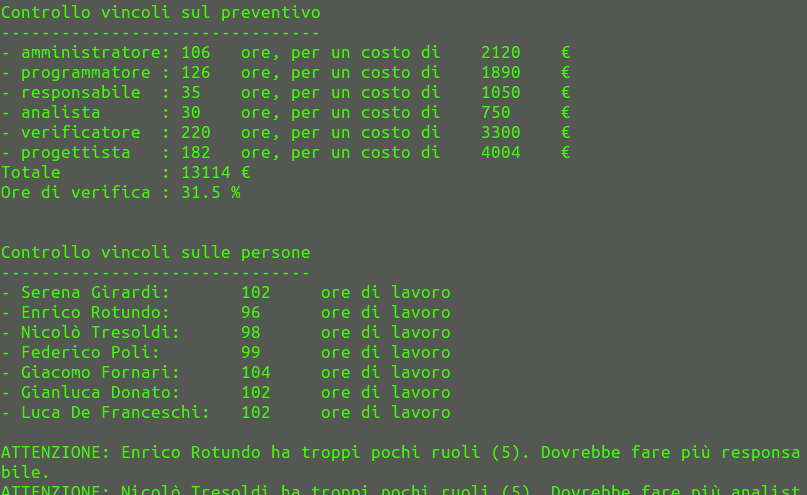
\includegraphics[scale=0.35] {ScriptGantt.png} 
    \caption{Esempio script}
\end{figure}

Per poterlo utilizzare, abilitare le API nel proprio account \glossario{TeamworkPM} per ottenere il token da utilizzare alla richiesta dello script. \\
Eseguirlo da terminale posizionandosi nella cartella \code{/PianoDiProgetto} con il comando \code{python download$\_$gantt.py}.

	\subsection{Ambiente di sviluppo}
		
		\subsubsection{Stesura del codice}
		
		Per la stesura del codice è consigliabile usare i seguenti editor:
		\begin{itemize}
			\item \textbf{gedit} $\geq 3.4.1$ (\url{http://projects.gnome.org/gedit})
			\item \textbf{Sublime text} $\geq 2.0.2$ (\url{http://www.sublimetext.com})
			\item \textbf{Eclipse} (\url{http://www.eclipse.org})
		\end{itemize}
		
		\subsubsection{Framework}
		
		Per lo sviluppo del progetto è previsto l'utilizzo del server \textbf{Node.js} $\geq 0.10.22$ e del relativo \glossario{package manager} \textbf{npm} $\geq 1.3.6$.

	\subsection{Ambiente di verifica e validazione}
	Gli strumenti utilizzati per effettuare l'analisi statica,dinamica e i test di unità descritti successivamente sono stati
	integrati in \glossario{Jenkins} v1.548 e ne è stata predisposta un'esecuzione automatica prima di effettuare \glossario{push}
	sul \glossario{repository}, in modo da garantire che le modifiche non introducano errori nel software esistente e che rispettino
	le metriche software riportate in \PianoDiQualifica{}.

		\subsubsection{Strumenti per l'analisi statica}
		
		Per l'analisi statica del codice Javascript e per aiutare a identificare automaticamente gli errori, sono integrati in
		Jenkins:
		\begin{itemize}
		\item \textbf{JSHint} (\url{http://www.jshint.com}),\glossario{tool} che aiuta a identificare gli errori e i potenziali
		problemi nel
		codice JavaScript.
		\item \textbf{JSLint} (\url{http://www.jslint.com}), \glossario{tool} usato per verificare se il codice JavaScript compila
		secondo le regole di linguaggio.
		\item \textbf{Closure Compiler} (\url{http://developers.google.com/closure/compiler}), \glossario{tool} utilizzato per
		rendere JavaScript più efficiente in termini di download e di esecuzione, migliorandolo rimuovendo \glossario{codice
		morto} , riscrivendolo e minimizzandolo. Controlla inoltre la sintassi, i riferimenti alle variabili, i tipi ed eventuali
		insidie.
		\end{itemize}
		
		\subsubsection{Strumenti per l'analisi dinamica} 
		Tool integrati in Jenkins per l'analisi dinamica: 
		\begin{itemize}
		\item \textbf{Mocha} (\url{https://github.com/visionmedia/mocha}) Mocha è una libreria ricca di funzionalità per l'esecuzione
		di test Javascript, con esecuzione di quest'ultimi asincrona ed in serie, permettendo segnalazioni flessibili ed accurate.
		\end{itemize}
	
			
		\subsubsection{Strumenti per la validazione}
		Per la validazione delle pagine web si utilizzeranno gli strumenti messi a disposizione da \glossario{W3C} alle pagine 
		 (\url{http://validator.w3.org}) e (\url{ http://jigsaw.w3.org/css-validator}).			
		
